\documentclass[review, authoryear]{elsarticle}

\usepackage{IEEEtrantools}
\usepackage{amsmath}
\usepackage{mathrsfs}
\usepackage{graphicx}
\usepackage{setspace}
\usepackage{amsfonts}
\usepackage{subfig}
\usepackage{float}
\floatstyle{plaintop}
\restylefloat{table}
\usepackage[noheads,nomarkers,tablesfirst]{endfloat}
\usepackage[utf8]{inputenc}
\usepackage{lineno}
\usepackage{fixltx2e}
\usepackage{natbib}
\usepackage{siunitx}

\begin{document}


\begin{frontmatter}

  \title{Forecasting the Ecology of the Red Sea using a Cluster of Regional
1D Marine Ecosystem Assimilative Models}

  \author[1]{Denis Dreano}

  \author[3]{George Triantafyllou}

  \author[3]{Kostas Tsiaras}

  \author[2]{Bani Mallick}
  
  \author[1]{Ibrahim Hoteit\corref{cor1}}
  \ead{ibrahim.hoteit@kaust.edu.sa} \cortext[cor1]{Corresponding author}


  \address[1]{Computer, Electrical and Mathematical Sciences and Engineering Division, King Abdullah University of Science and Technology}

  \address[2]{Department of Statistics, Texas A\&M University}

  \address[3]{Hellenic Center for Marine Research}

  \begin{abstract}
  Abstract
  \end{abstract}

\end{frontmatter}

\linenumbers

\section{Introduction}

\paragraph{3D marine ecological models...}

\begin{itemize}
  \item marine ecology models represent biogeochemical interactions as
differential equations.
  \item Can be as minimal as NPZ or as complete as NPZ
\end{itemize}

\paragraph{...are useful because...}

\begin{itemize}
  \item HAB affect public health, desalination and coastal economy
  \item predicting chlorophyll can help fisheries
  \item For research: better understand the large-scale ecosystem
  \item Especially usefull because we lack data about the subsurface
phenomena
\end{itemize}

\paragraph{...But expensive and difficult to run}

\begin{itemize}
  \item \citep{Anderson2005} lot of underdetermination
  \item circulation model very expensive, because very small grid
\end{itemize}

\paragraph{In this article we look at ways to simulate 3D ecosystems more
cheaply by running many parallel 1D regional models}

\begin{itemize}
  \item Divide the Red sea in small regions with similar ecology
  \item Reduces underdetermination
  \item Ensure parametrization is better for each region
\end{itemize}

\paragraph{We are going to test that idea on the Red Sea because...}

\begin{itemize}
  \item Red Sea is an interesting environment: extreme temperatures and
salinity
  \item Very rich and preserved ecosystem
  \item Unexplored environment
  \item Lack of data: therefore developing models is important
\end{itemize}

\paragraph{We will use the hybrid-SEIK data assimilation scheme, because...}

\begin{itemize}
  \item Assimilation constrains the model and reduces underdetermination
  \item Mitigates the fact that initial conditions are unknown
  \item SEIK is better than SEEK for strongly nonlinear models
  \item SEIK is better than EnKF when fewer observations than states
  \item hybridization reduces the ensemble size and the computational cost
\end{itemize}

\paragraph{We will assimilate Chl data even if it is imperfect because it is
the best available data for the Red Sea}

\begin{itemize}
  \item Chl data allows to observe large scale ecological patterns with
high spatial and temporal coverage.
  \item Compared with in situ data that are limited in time and space,
and expensive.
  \item However chl data suffers from missing values due clouds, aerosols, etc.
  \item Also bad values near the coast, case II waters
  \item Both problem particularly affect the southern Red Sea, that has
nearly no observation in the summer during some months.
  \item However as lack of in situ data, this is the best we have
currently in the Red Sea
\end{itemize}

\paragraph{What we are going to do in this paper step by step}

\paragraph{What is new in this paper and why}

\paragraph{Introduce sections}


% 
% \paragraph{What are marine ecosystem models}
% ERSEM, NPZ.
% 
% \paragraph{Marine ecosystem models have scientific and practical applications}
% Forecasting, harmful algae blooms, scientific inquiry when not enough data.
% 
% \paragraph{Complex 3D ecological models have limitations}
% Indetermination and computational cost.
% 
% \paragraph{Assimilation in necessary but increases the computational cost}
% Ecological systems are chaotic system that require assimilation to
% maintain a good prediction skill. But assimilation increases the computational
% cost. Assimilation of eco models remains a challenge.
% 
% \paragraph{The hybrid-SEIK}
% Has never been use for eco models before.
% 
% \paragraph{Ocean colour data has been assimilated a lot to eco models}
% chlorophyll is a green colored pigment critical for photosynthesis and found
% in plants and algae \citep{Pal2014}. Give a detectable green coloration
% to the water when phytoplankton is present \citep{Robinson2010}.
% Remotely sensed ocean colour data give highly available data with 
% high coverage both in time and space \citep{Robinson2010}. Ocean colour
% data products like chl are very good proxy for phytoplankton concentration.
% 
% \paragraph{But has some limitations}
% CHL dataset have missing data because of clouds. Which is a big problem in 
% the southern Red Sea in summer where the coverage is almost zero
% \cite{Racault}. Moreover the chl is difficult to estimate in case II
% optically complex waters, especially near the caosts. It also particularly
% affects the southern Red Sea which is very shallow.
% 
% \paragraph{The Red Sea is a relatively unexplored sea}
% Not a lot of studies, not a lot of in situ data.
% Must use models and remotely-sensed data.
% RS is TTS with strong stratification that limits vertical diffusion of nutrients.
% \citep{Mann2006}.
% Other than the gulf of Aden \citep{Yao2015}, 
% the RS has no known significant input of nutrients and
% is oligotrophic \citep{Raitsos2013, Weikert1987}.
% Red Sea has a rich ecosystem and unique ecosystem that has adapted its
% extreme environment \citep{Raitsos2011}.
% RS relatively well preserved but increasingly fragilized by human activities.
% Sharp increase of temperature in the past decade threatend the RS environment.
% \citep{Raitsos2011}.
% 
% \paragraph{Major biological patterns}
% Current hypotheses about primary production in Red Sea.
% There is a lack of missing data therefore the large scale ecological 
% dynamics is poorly known \citep{Raitsos2013, Triantafyllou2014}.
% The role of aerosol deposition could be important but has not been investigated
% yet \citep{Raitsos2013}.
% Eddies are believed to play important role \citep{Raitsos2013, Zhan2014}.
% Chlorophyll increase from north to south \citep{Raitsos2013}.
% Secondary summer bloom (but not in NRS) \citep{Raitsos2013}.
% Strong Interannual variability \citep{Raitsos2013}.
% Exchange of water with GOA is a major driver of productivity for the 
% whole Red Sea \citep{Triantafyllou2014}.
% SRS winter bloom attributed to wind-driven intrusion \citep{Raitsos2013}.
% Deep convection in winter plays a big role in the northern Red Sea
% \citep{Raitsos2013}.
% Red Sea circulation impacted by eddies that could impact productivity
% \citep{Zhai2013}. Central red Sea anti cyclonic eddy is believed to
% control June peak \citep{Raitsos2013}.
% Climate mode indices have impact ton the Red Sea \citep{Raitsos2015}.
% 
% 
% \paragraph{Objective:}
% 3D ecological models are expensive to run. Can we divide the Red Sea into
% regions and have 1D models running in each of them in parallel?
% In this article we cluster the Red Sea in 3 different eco-regions using
% automatic unsupervised learning algorithms. We then run an assimilative 1D
% ecological model on each of the region and analyze the results.
% 
% \paragraph{Introduce chapters}


\newcommand{\cov}{\text{cov}}

\newcommand{\0}{\mathbf{0}}

\newcommand{\C}{\mathbf{C}}
%\newcommand{\A}{\mathbf{A}}
\newcommand{\X}{\mathbf{X}}
\newcommand{\U}{\mathbf{U}}
\renewcommand{\V}{\mathbf{V}}
\newcommand{\M}{\mathbf{M}}
\newcommand{\Q}{\mathbf{Q}}
\renewcommand{\H}{\mathbf{H}}
\newcommand{\I}{\mathbf{I}}
%\newcommand{\K}{\mathbf{K}}
%\newcommand{\W}{\mathbf{W}}
\newcommand{\R}{\mathbf{R}}
%\newcommand{\N}{\mathbf{N}}
\renewcommand{\P}{\mathbf{P}}
\renewcommand{\L}{\mathbf{L}}

\renewcommand{\a}{\mathbf{a}}
\newcommand{\h}{\mathbf{h}}
\renewcommand{\r}{\mathbf{r}}
\newcommand{\x}{\mathbf{x}}
%\newcommand{\s}{\mathbf{s}}
\renewcommand{\k}{\mathbf{k}}
\newcommand{\y}{\mathbf{y}}
\newcommand{\z}{\mathbf{z}}

\newcommand{\SSigma}{\mathbf{\Sigma}}
\newcommand{\GGamma}{\mathbf{\Gamma}}

\newcommand{\ttheta}{\boldsymbol\theta}
\newcommand{\eeta}{\boldsymbol\eta}
\newcommand{\vvarepsilon}{\boldsymbol\varepsilon}
\newcommand{\xxi}{\boldsymbol\xi}
\newcommand{\mmu}{\boldsymbol\mu}

\section{Data}

\subsection{Chlorophyll data}

We use CCI monthly and 8-days CHL data.

\begin{quotation}

Satellite data provide chlorophyll (CHL) concentrations with a spatial and
temporal resolution not achievable with in situ observations, making them
particularly relevant to the Red Sea, where very few in situ data collection
are conducted.

Level-3 mapped data from the NASA \mbox{SeaWiFS} (Sea-Viewing Wide
Field-of-View Sensor) satellite sensor are used in this study. The dataset is
publicly available at \texttt{http://oceancolor.gsfc.nasa.gov}. In this study,
we use the 9km resolution mapped weekly averages from January 1998 to December
2007 (460 time steps). At each time step, a $133\times 188$ pixel map is
available for a domain extending from longitudes between $33^\circ$E and
$44^\circ$E and latitudes between $12^\circ$N and $28^\circ$N, of which 5635
pixels correspond to actual Red Sea surface (see Figure \ref{figure1}(a)). A
log-transformation was applied in order to obtain an approximately Gaussian
distribution \cite{Campbell1995}. Pixels with too few observations were
discarded, and a control quality check was applied to remove outliers
\cite{Willis2004}.

Remotely sensed CHL may have missing data because of cloud coverage. The cloud
variability in the Red Sea follows a seasonal cycle. Figure \ref{figure1}(c)
shows that the cloud coverage is particularly pronounced during summers because
of the monsoon and it is sparse during winters. The cloud coverage is, however,
not homogenous over the Red Sea. It is much more pronounced in the south
(figure \ref{figure1}(b)). In this region, almost no data are available during
summers.

%\begin{figure}[h] \centering \includegraphics{../png/figure1.png} \caption{Raw
%data plots: (a) map of average log-concentrations of CHL between 1998 and 2004,
%(b) map of average percentage of missing data for each location between 1998
%and 2006, and (c) time-series of the percentage of missing data over the Red
%Sea between 1998 and 2004.} \label{figure1} \end{figure}


\end{quotation}

\subsection{DINEOF}

CCI data present missing data, in particular, in the southern Red Sea during
summer. In order to have a complete dataset on which can apply a clustering
algorithm, we use DINEOF, a data filling algorithm. The Chl data is averaged
over each region to give a data time-series for each of them.

\begin{quotation} The DINEOF (Data Interpolating Empirical Orthogonal Function)
is an EOF-based, recursive method for the reconstruction of data matrices with
missing values \cite{Beckers2003, Alvera-Azcarate2009}. It estimates the values
of the missing data by successive singular values decompositions (SVD) of a
given data matrix and truncated reconstructions. The advantage of this method
is that it does not require any a priori information about the data. It has
been successfully used for reconstruction of incomplete chlorophyll datasets in
different regions of the ocean \cite{Miles2010,Sirjacobs2011,Waite2013}.

Let $\X$ be an $m \times k$ centered data matrix with missing values initially
filled with 0s.  Then, until the missing values have converged, the following
steps are repeated. An SVD is first applied to the data matrix: $\X = \U\SSigma
\V^T$, with $\U$ an $m\times m$ unitary matrix, $\SSigma$ an $m\times k$
diagonal matrix and $\V$ a $k\times k$ unitary matrix. The missing values are
then replaced by the truncated reconstruction order $n$ of the data matrix:
$\{\X\}_{i,j} = \{\U^{(n)}\SSigma^{(n)} (\V^{(n)})^T)\}_{i,j}$, for $i,j$
indices of the missing values, with $\U^{(n)}$ the $m\times n$ matrix composed
of the $n$ first columns of $\U$, $\V^{(n)}$ the $k\times n$ matrix composed of
the $n$ first columns of $\V$, and $\SSigma^{(n)}$ the $n\times n$ diagonal
matrix with the $n$ largest eigenvalues on its diagonal. It is assumed that the
eigenvalues and eigenvector are sorted by decreasing order of eigenvalues. In
\cite{Alvera-Azcarate2009}, the authors introduced the filtering of the
temporal covariance matrix as a way of reducing spurious oscillations that may
appear when the data are sparsely sampled in time. This filtering is controlled
by the parameter of the Laplacian filter and the number of times the filter is
applied.

The values of the DINEOF parameters are determined following the method
outlined in \cite{Alvera-Azcarate2009}. The smoothing parameter of the
Laplacian filter is set to 0.005. The number of modes in the truncation and the
number of times the filter is applied are chosen following a cross-validation
technique. A random subset of observed values is taken from $X$ and assumed to
be missing before the DINEOF is applied. The algorithm is then run with
different numbers of iterations (1, 3, 10, 30, 100) and orders of truncation
(from 2 to 50). The set of parameters minimizing the RMS error over the
cross-validation data is chosen as the best number of iterations and order of
truncation. The approach of \cite{Beckers2006} is followed to select a
cross-validation dataset. Instead of selecting it by sampling the dataset point
by point, contiguous regions are set aside. These regions correspond to regions
of missing data from the original dataset and are selected randomly until 3\%
of the data have been extracted.

\end{quotation}

\subsection{Clustering}

We use clustering algorithm to divide the Red Sea into regions with similar
behavior. We tried K-means and Gaussian Mixture Model, a generalization of the
former.GMM was found to give better results.

\begin{quotation} I used clustering algorithms in order to derive the Red Sea
eco-regions. These were applied to monthly log-concentration of chlorophyll. I
used SeaWiFS data, that has been filled using DINEOF. I used the popular
K-means, and the Gaussian Mixture Model (GMM) clustering algorithms.

I found that GMM provides more robust results. With any number of clusters, we
obtain a division of the Red Sea into regions of comparable sizes.  With 5
clusters, the regions (shown in figure \ref{cluster}) are very similar to those
identified by \citet{Raitsos2013}.  Contrary to the purely latitudinal division
proposed by the former, we observe that the separation between clusters is
curved at the position of major Red Sea eddies.  The fact that the curvature is
oriented toward the south suggests that most nutrients propagate northward from
the Gulf of Aden.

%\begin{figure}[h] \centering
%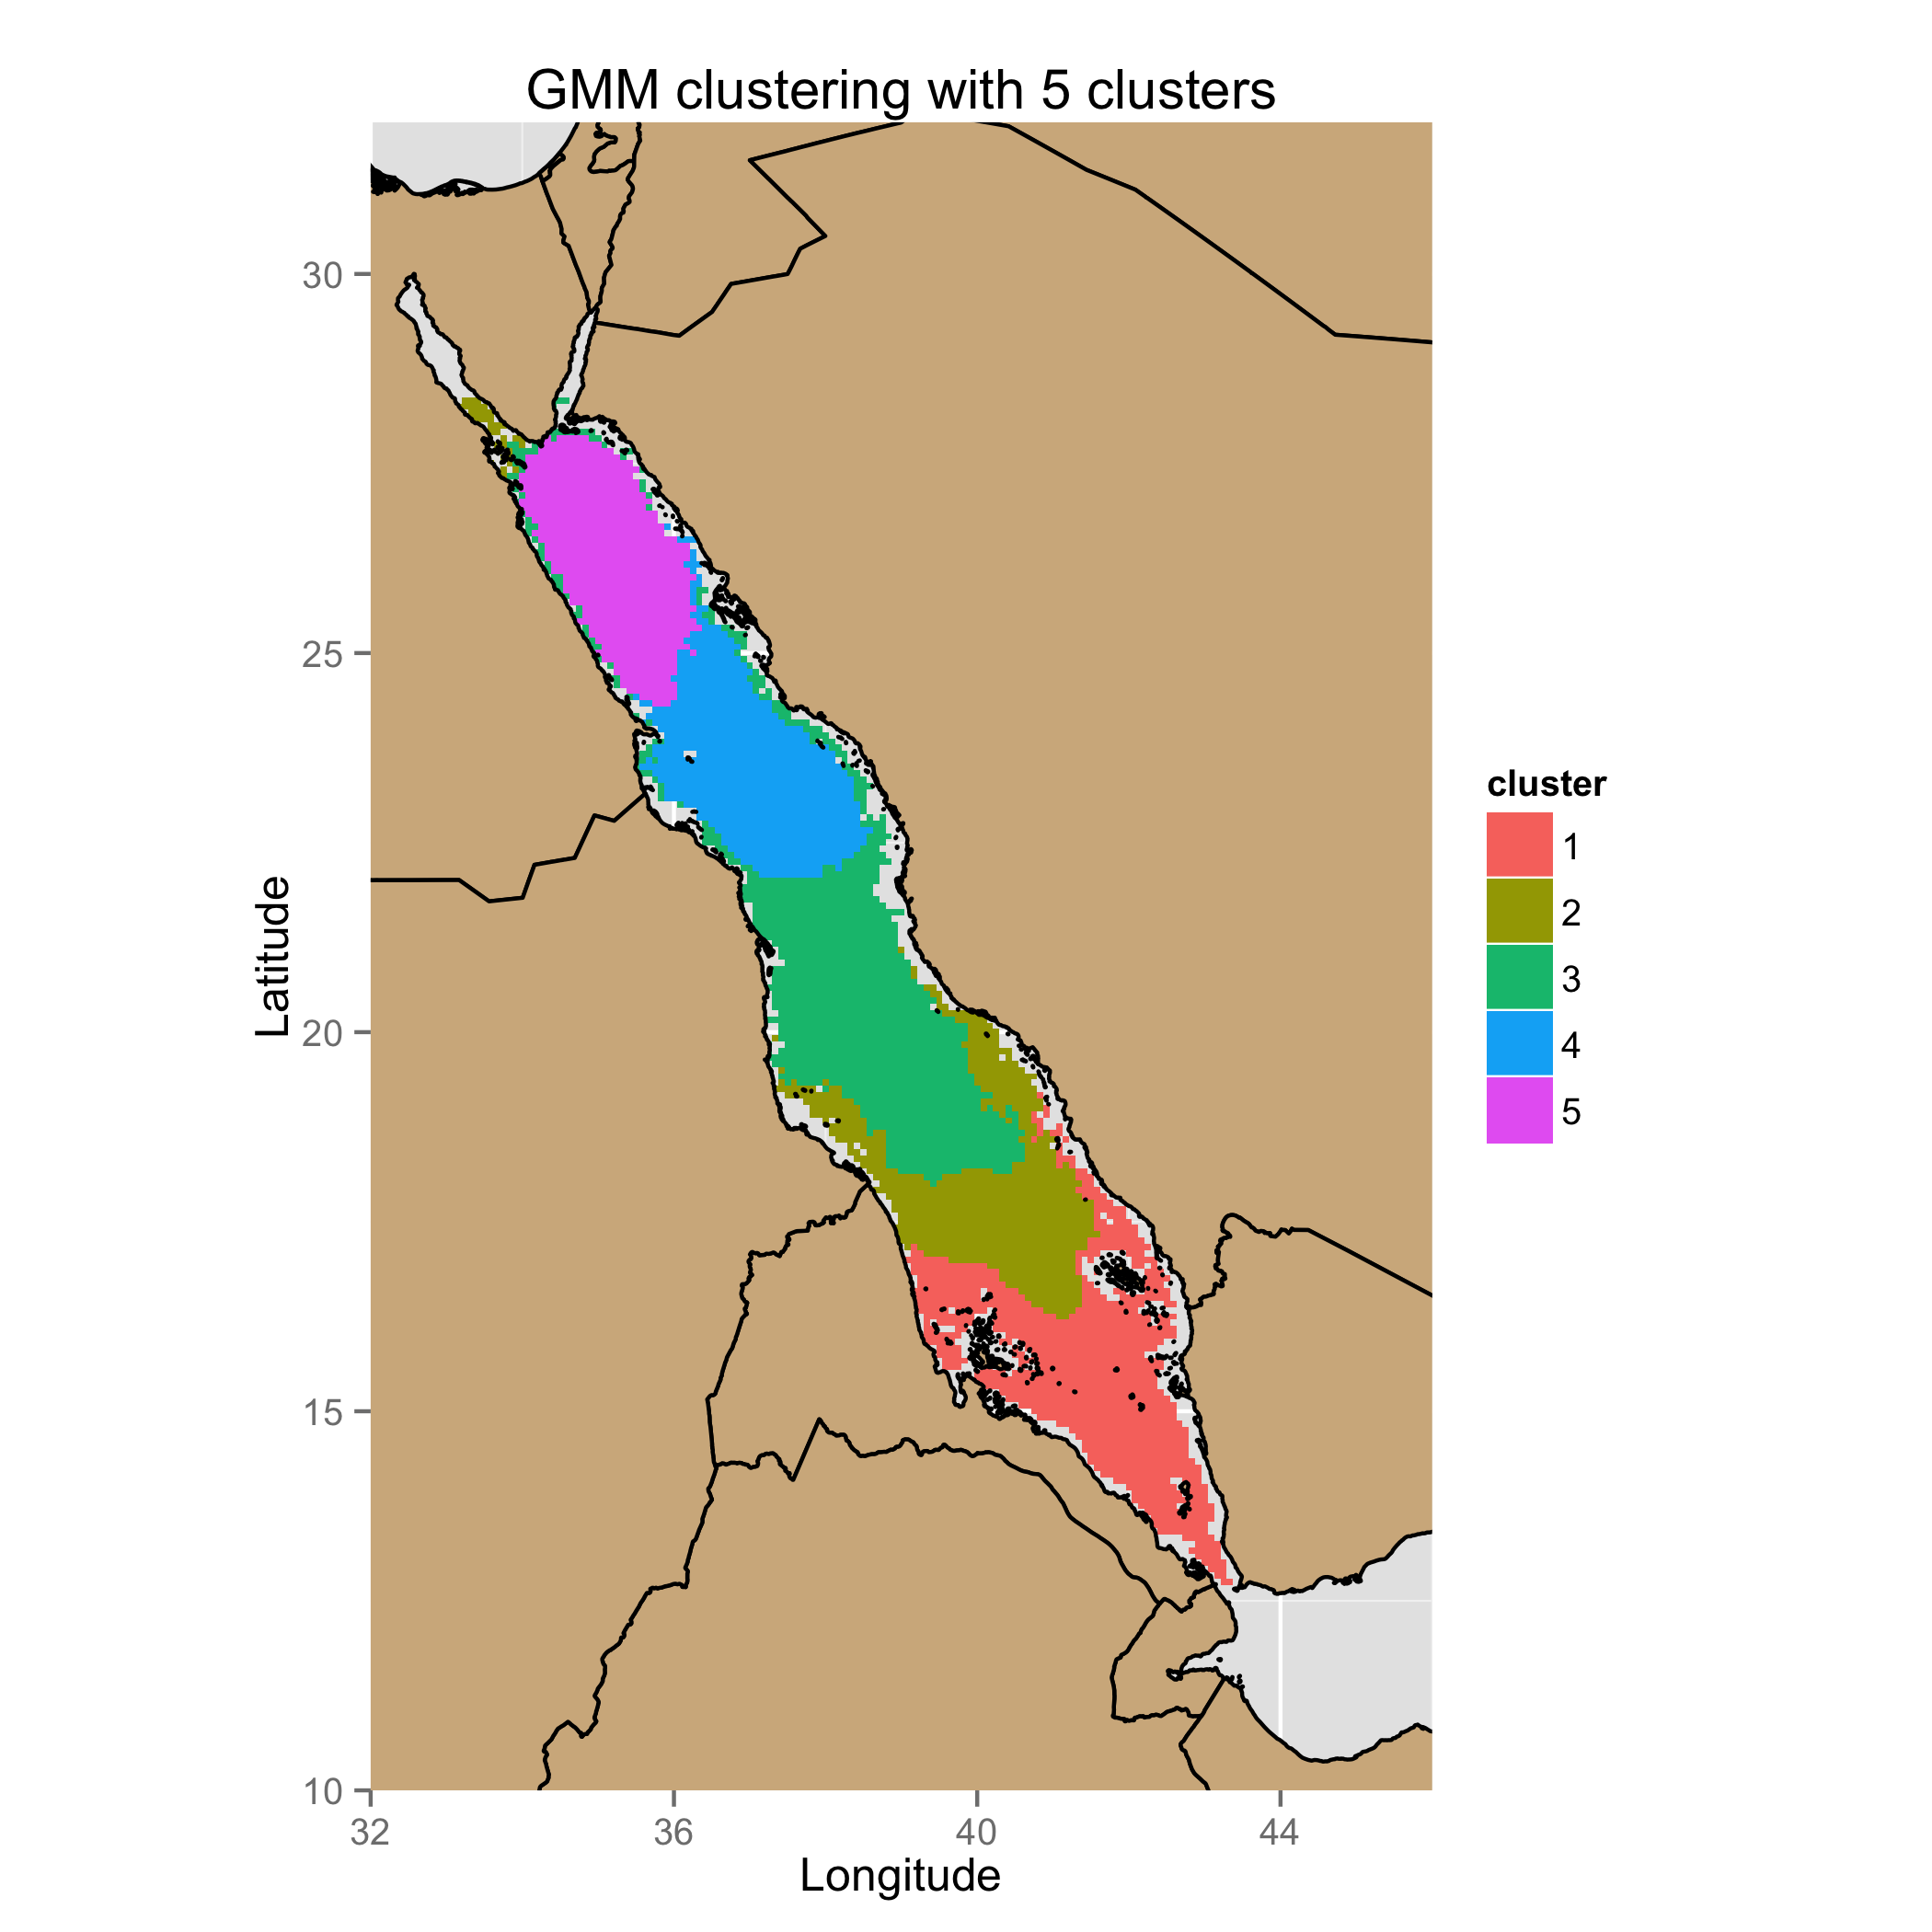
\includegraphics[scale=.15]{figures/clusters_k5.png} \caption{Clustering of Red
%Sea using GMM, with filled monthly SeaWiFS chlorophyll data.} \label{cluster}
%\end{figure}

In Chapter 2, I plan to use the dataset constructed in Chapter 1.  By using CCI
chlorophyll data instead of SeaWiFS, the need for data filling is minimized.
This is desirable, as data filling can introduce biases. It will also be
possible to use additional variables. For example, we can expect the
temperature and the bathymetry to have a large impact on the Red Sea
phytoplankton biology. Sea level anomaly can be useful in that it indicates the
presence of mesoscale eddies. Finally, alternative clustering algorithms will
be tested.  \end{quotation}



\section{Model and Assimilation}

\subsection{1D-ERSEM model}

\paragraph{Description of ERSEM}

\paragraph{Initialization/Parameters/Forcing}

\subsection{Data Assimilation}

\paragraph{We chose hybrid-SEIK DA scheme because...}

\paragraph{Equations of hybrid-SEIK}

\paragraph{Parameters}


\section{Results}

\subsection{Model evaluation}

Here, we compare the results of the free-run with the assimilated-run.
We show that we have a good prediction skill, and that the assimilation
improves the model.

\paragraph{Plot some models output vs the data and qualitative comments}

\paragraph{Discuss different metrics to evaluate model and DA schemes}

\paragraph{Show a couple metrics on our results}

\subsection{Analysis}

Here we look at the results and interpret them biologycally. Do we find
comparable results as Acker, Raitsos, Weiker, etc. What can we say about the
hypothesis that they made about he process that drive primary productivity in
the Red Sea.

\paragraph{Discuss differences between climatology and 2003-2004}

\paragraph{Comment on the role of overturning and stratification}

\paragraph{What is the limiting nutrient?}

$$\frac{N3N + N4N}{N1P}$$
vs Redfied ratio

\paragraph{Compute production at different time of years and compare
with Weikert1987/Acker2008/Koblentz}

\paragraph{Study the DCM}


\section{Conclusion}

Summary of the proposed approach

Are several 1D paralled 1D models a good alternative to 3D simulations?

What did we learn about the Red Sea ecology?

Future works?


\section*{Acknowledgment}

The research reported in this publication was supported by King Abdullah
University of Science and Technology (KAUST).

\section{Bibliography}

\bibliographystyle{agufull08} \bibliography{References}

\end{document}